\documentclass{beamer}
\usepackage[utf8]{inputenc}
\usetheme{Madrid}
\usecolortheme{default}
\usepackage{amsmath,amssymb,amsfonts,amsthm}
\usepackage{txfonts}
\usepackage{tkz-euclide}
\usepackage{listings}
\usepackage{adjustbox}
\usepackage{array}
\usepackage{tabularx}
\usepackage{gvv}
\usepackage{lmodern}
\usepackage{circuitikz}
\usepackage{tikz}
\usepackage{graphicx}

\setbeamertemplate{page number in head/foot}[totalframenumber]

\usepackage{tcolorbox}
\tcbuselibrary{minted,breakable,xparse,skins}



\definecolor{bg}{gray}{0.95}
\DeclareTCBListing{mintedbox}{O{}m!O{}}{%
  breakable=true,
  listing engine=minted,
  listing only,
  minted language=#2,
  minted style=default,
  minted options={%
    linenos,
    gobble=0,
    breaklines=true,
    breakafter=,,
    fontsize=\small,
    numbersep=8pt,
    #1},
  boxsep=0pt,
  left skip=0pt,
  right skip=0pt,
  left=25pt,
  right=0pt,
  top=3pt,
  bottom=3pt,
  arc=5pt,
  leftrule=0pt,
  rightrule=0pt,
  bottomrule=2pt,
  toprule=2pt,
  colback=bg,
  colframe=orange!70,
  enhanced,
  overlay={%
    \begin{tcbclipinterior}
    \fill[orange!20!white] (frame.south west) rectangle ([xshift=20pt]frame.north west);
    \end{tcbclipinterior}},
  #3,
}
\lstset{
    language=C,
    basicstyle=\ttfamily\small,
    keywordstyle=\color{blue},
    stringstyle=\color{orange},
    commentstyle=\color{green!60!black},
    numbers=left,
    numberstyle=\tiny\color{gray},
    breaklines=true,
    showstringspaces=false,
}
%------------------------------------------------------------
%This block of code defines the information to appear in the
%Title page
\title %optional
{4.8.32}

%\subtitle{A short story}

\author % (optional)
{AI25BTECH11036-SNEHAMRUDULA}



\begin{document}


\frame{\titlepage}
\begin{frame}{Question}
 Find the projection of vector $(\vec{b}+\vec{c})$ on vector $\vec{a}$, where 
\begin{align}
\vec{a} = 2\hat{i} + 2\hat{j} + \hat{k}, \quad 
\vec{b} = \hat{i} + 3\hat{j} + \hat{k}, \quad 
\vec{c} = \hat{i} + \hat{k}.
\end{align}\\ 
\end{frame}
\begin{frame}{Theoretical Solution}
Let us solve the given equation theoretically and then verify the solution computationally \\
According to the question, \\
Given three vectors\\
\begin{align}
\vec{a}=\begin{myvec}{2\\2\\1}\end{myvec}\
\vec{b}=\begin{myvec}{1\\3\\1}\end{myvec}\
\vec{c}=\begin{myvec}{1\\0\\1}\end{myvec}\
\end{align}
   \begin{align}
 \vec{b}+\vec{c}=\begin{myvec}{2\\3\\2}\end{myvec}
\end{align}
Projection of vector ($\vec{b}+\vec{c}$) is k$\frac{\vec{a}}{\|\vec{a}\|}$
\begin{align}
    K=\frac{(\vec{b}+\vec{c})^T\vec{a}}{\|\vec{a}\|}=4
\end{align}
\end{frame}
\begin{frame}{Theoretical Solution}
\begin{align}
\text{Projection of vector } (\vec{b}+\vec{c}) = 
\begin{pmatrix}
2.67 \\
2.67 \\
1.33
\end{pmatrix}
\end{align}
\end{frame}

\begin{frame}{Plot}
    \centering
    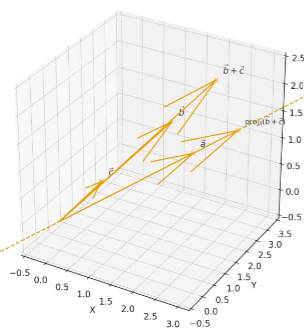
\includegraphics[width=\columnwidth, height=0.8\textheight, keepaspectratio]{4.8.32.png}     
\end{frame}
\end{document}
